\documentclass[12pt]{article}
%%---------------------------------------------------------------------
% packages
% geometry
\usepackage{geometry}
% font
\usepackage{fontspec}
\defaultfontfeatures{Mapping=tex-text}  %%如果没有它,会有一些 tex 特殊字符无法正常使用,比如连字符。
\usepackage{xunicode,xltxtra}
\usepackage[BoldFont,SlantFont,CJKnumber,CJKchecksingle]{xeCJK}  % \CJKnumber{12345}: 一万二千三百四十五
\usepackage{CJKfntef}  %%实现对汉字加点、下划线等。
\usepackage{pifont}  % \ding{}
% math
\usepackage{amsmath,amsfonts,amssymb}
% color
\usepackage{color}
\usepackage{xcolor}
\definecolor{EYE}{RGB}{199,237,204}
\definecolor{FLY}{RGB}{128,0,128}
\definecolor{ZHY}{RGB}{139,0,255}
% graphics
\usepackage[americaninductors,europeanresistors]{circuitikz}
\usepackage{tikz}
\usetikzlibrary{positioning,arrows,shadows,shapes,calc,mindmap,trees,backgrounds}  % placements=positioning
\usepackage{graphicx}  % \includegraphics[]{}
\usepackage{subfigure}  %%图形或表格并排排列
\usepackage{fancyvrb}
\usepackage{listings}%代码高亮
\lstset{language=C++}%这条命令可以让LaTeX排版时将C++键字突出显示
\lstset{breaklines}%这条命令可以让LaTeX自动将长的代码行换行排版
\lstset{extendedchars=false}
% table
\usepackage{colortbl,dcolumn}  %% 彩色表格
\usepackage{multirow}
\usepackage{multicol}
\usepackage{booktabs}
% code
\usepackage{fancyvrb}
\usepackage{listings}
% title
\usepackage{titlesec}
% head/foot
\usepackage{fancyhdr}
% ref
\usepackage{hyperref}
% pagecolor
\usepackage[pagecolor={EYE}]{pagecolor}
% tightly-packed lists
\usepackage{mdwlist}

\usepackage{styles/iplouccfg}
\usepackage{styles/zhfontcfg}
\usepackage{styles/iplouclistings}

%%---------------------------------------------------------------------
% settings
% geometry
\geometry{left=2cm,right=1cm,top=2cm,bottom=2cm}  %设置 上、左、下、右 页边距
\linespread{1.5} %行间距
% font
\setCJKmainfont{Adobe Kaiti Std}
%\setmainfont[BoldFont=Adobe Garamond Pro Bold]{Apple Garamond}  % 英文字体
%\setmainfont[BoldFont=Adobe Garamond Pro Bold,SmallCapsFont=Apple Garamond,SmallCapsFeatures={Scale=0.7}]{Apple Garamond}  %%苹果字体没有SmallCaps
\setCJKmonofont{Adobe Fangsong Std}
% graphics
\graphicspath{{figures/}}
\tikzset{
    % Define standard arrow tip
    >=stealth',
    % Define style for boxes
    punkt/.style={
           rectangle,
           rounded corners,
           draw=black, very thick,
           text width=6.5em,
           minimum height=2em,
           text centered},
    % Define arrow style
    pil/.style={
           ->,
           thick,
           shorten <=2pt,
           shorten >=2pt,},
    % Define style for FlyZhyBall
    FlyZhyBall/.style={
      circle,
      minimum size=6mm,
      inner sep=0.5pt,
      ball color=red!50!blue,
      text=white,},
    % Define style for FlyZhyRectangle
    FlyZhyRectangle/.style={
      rectangle,
      rounded corners,
      minimum size=6mm,
      ball color=red!50!blue,
      text=white,},
    % Define style for zhyfly
    zhyfly/.style={
      rectangle,
      rounded corners,
      minimum size=6mm,
      ball color=red!25!blue,
      text=white,},
    % Define style for new rectangle
    nrectangle/.style={
      rectangle,
      draw=#1!50,
      fill=#1!20,
      minimum size=5mm,
      inner sep=0.1pt,}
}
\ctikzset{
  bipoles/length=.8cm
}
% code
\lstnewenvironment{VHDLcode}[1][]{%
  \lstset{
    basicstyle=\footnotesize\ttfamily\color{black},%
    columns=flexible,%
    framexleftmargin=.7mm,frame=shadowbox,%
    rulesepcolor=\color{blue},%
%    frame=single,%
    backgroundcolor=\color{yellow!20},%
    xleftmargin=1.2\fboxsep,%
    xrightmargin=.7\fboxsep,%
    numbers=left,numberstyle=\tiny\color{blue},%
    numberblanklines=false,numbersep=7pt,%
    language=VHDL%
    }\lstset{#1}}{}
\lstnewenvironment{VHDLmiddle}[1][]{%
  \lstset{
    basicstyle=\scriptsize\ttfamily\color{black},%
    columns=flexible,%
    framexleftmargin=.7mm,frame=shadowbox,%
    rulesepcolor=\color{blue},%
%    frame=single,%
    backgroundcolor=\color{yellow!20},%
    xleftmargin=1.2\fboxsep,%
    xrightmargin=.7\fboxsep,%
    numbers=left,numberstyle=\tiny\color{blue},%
    numberblanklines=false,numbersep=7pt,%
    language=VHDL%
    }\lstset{#1}}{}
\lstnewenvironment{VHDLsmall}[1][]{%
  \lstset{
    basicstyle=\tiny\ttfamily\color{black},%
    columns=flexible,%
    framexleftmargin=.7mm,frame=shadowbox,%
    rulesepcolor=\color{blue},%
%    frame=single,%
    backgroundcolor=\color{yellow!20},%
    xleftmargin=1.2\fboxsep,%
    xrightmargin=.7\fboxsep,%
    numbers=left,numberstyle=\tiny\color{blue},%
    numberblanklines=false,numbersep=7pt,%
    language=VHDL%
    }\lstset{#1}}{}
% pdf
\hypersetup{pdfpagemode=FullScreen,%
            pdfauthor={Haiyong Zheng},%
            pdftitle={Title},%
            CJKbookmarks=true,%
            bookmarksnumbered=true,%
            bookmarksopen=false,%
            plainpages=false,%
            colorlinks=true,%
            citecolor=green,%
            filecolor=magenta,%
            linkcolor=cyan,%red(default)
            urlcolor=cyan}
% section
%http://tex.stackexchange.com/questions/34288/how-to-place-a-shaded-box-around-a-section-label-and-name
\newcommand\titlebar{%
\tikz[baseline,trim left=3.1cm,trim right=3cm] {
    \fill [cyan!25] (2.5cm,-1ex) rectangle (\textwidth+3.1cm,2.5ex);
    \node [
        fill=cyan!60!white,
        anchor= base east,
        rounded rectangle,
        minimum height=3.5ex] at (3cm,0) {
        \textbf{\thesection.}
    };
}%
}
\titleformat{\section}{\Large\bf\color{blue}}{\titlebar}{0.1cm}{}
% head/foot
\setlength{\headheight}{15pt}
\pagestyle{fancy}
\fancyhf{}

\chead{\color{black!50!green}Camtasia Studio 使用指南}

\lfoot{\color{blue!50!green}}
\cfoot{\color{blue!50!green}\href{http://vision.ouc.edu.cn/~zhenghaiyong}{CVBIOUC}}
\rfoot{\color{blue!50!green}$\cdot$\ \thepage\ $\cdot$}
\renewcommand{\headrulewidth}{0.4pt}
\renewcommand{\footrulewidth}{0.4pt}

%%---------------------------------------------------------------------
\begin{document}
%%---------------------------------------------------------------------
%%---------------------------------------------------------------------
% \titlepage
\title{Camtasia Studio 使用指南}
\author{CVBIOUC}
%\date{\vspace{-0.7em}December 26th, 2014\vspace{-0.7em}}
%%---------------------------------------------------------------------
\maketitle\thispagestyle{fancy}
%%---------------------------------------------------------------------
\maketitle
%\tableofcontents 

\section{录制准备工作}
1. 打开Camtasia Studio 软件,选择{\color{blue}{录制屏幕}}选项(如图~\ref{fig:fig1}所示)。
    \begin{figure}[!ht]
    \centering
    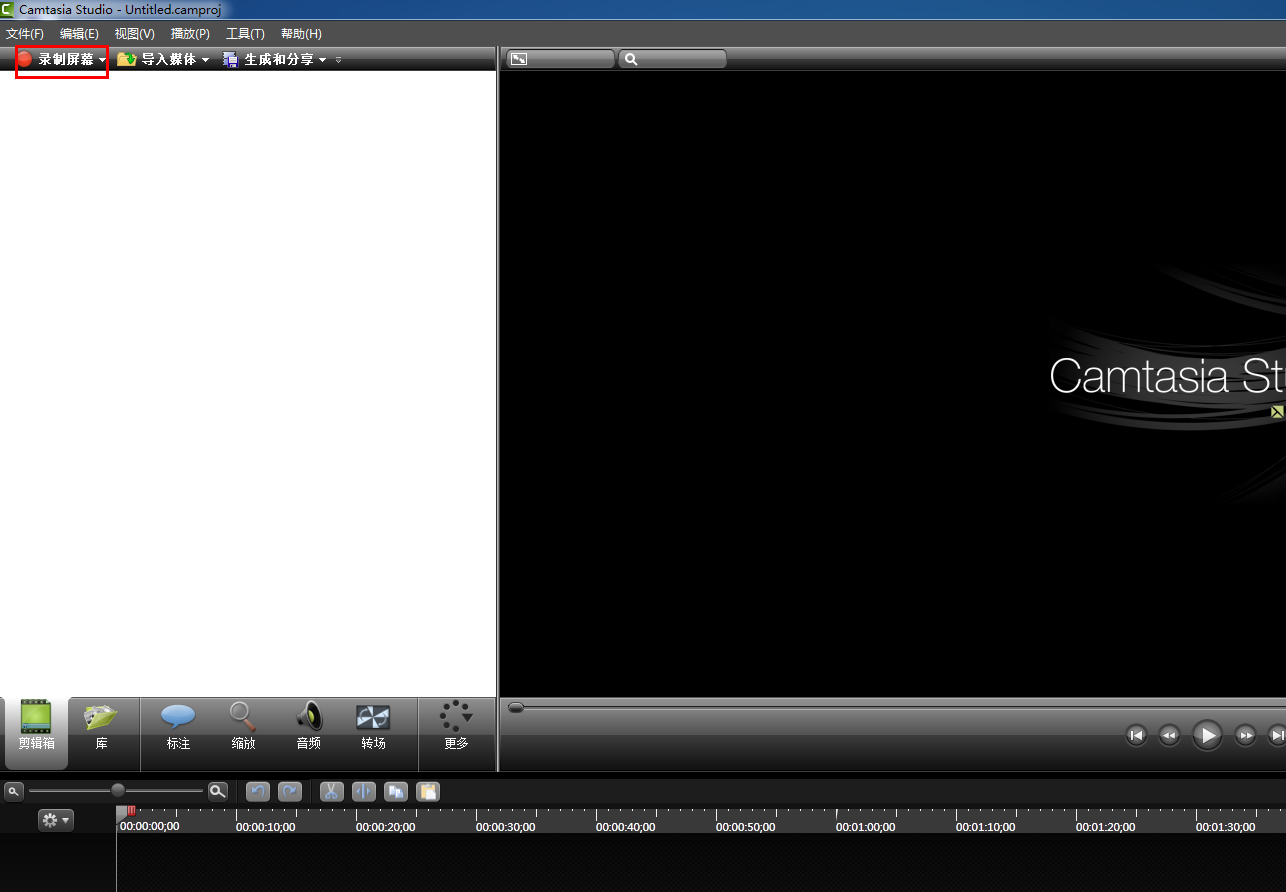
\includegraphics[width=0.9\textwidth]{fig1.png}
    \caption{选择录制屏幕}
    \label{fig:fig1}
    \end{figure}  
    
2. 设置录像参数(如图~\ref{fig:fig2}所示),选择区域设置为{\color{blue}{全屏幕}},录制音频设置为(如图~\ref{fig:fig3}所示)。
    \begin{figure}[!ht]
    \centering
    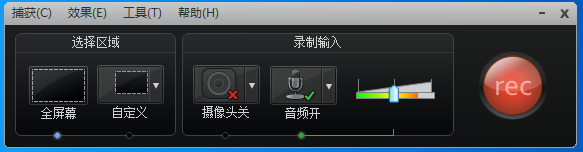
\includegraphics[width=0.5\textwidth]{fig2.png}
    \caption{设置录像参数}
    \label{fig:fig2}
    \end{figure}  
    \begin{figure}[!ht]
    \centering
    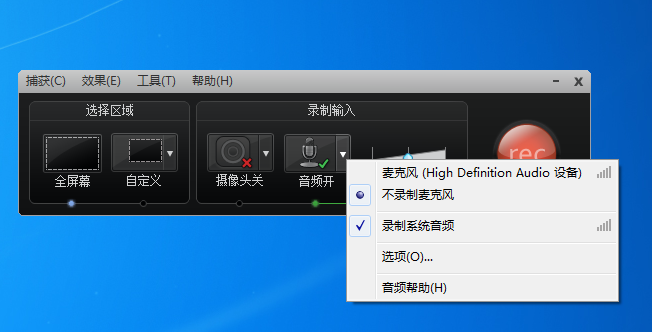
\includegraphics[width=0.5\textwidth]{fig3.png}
    \caption{设置录制音频}
    \label{fig:fig3}
    \end{figure} 
\section{录制}
1. 点击{\color{blue}{rec}}开始录制。\par
2. 点击{\color{blue}{F10}}停止录制。\par
3. 点击{\color{blue}{保存并编辑}},保存录制文件(xxxx.trec),如图~\ref{fig:fig4}所示。
    \begin{figure}[!ht]
    \centering
    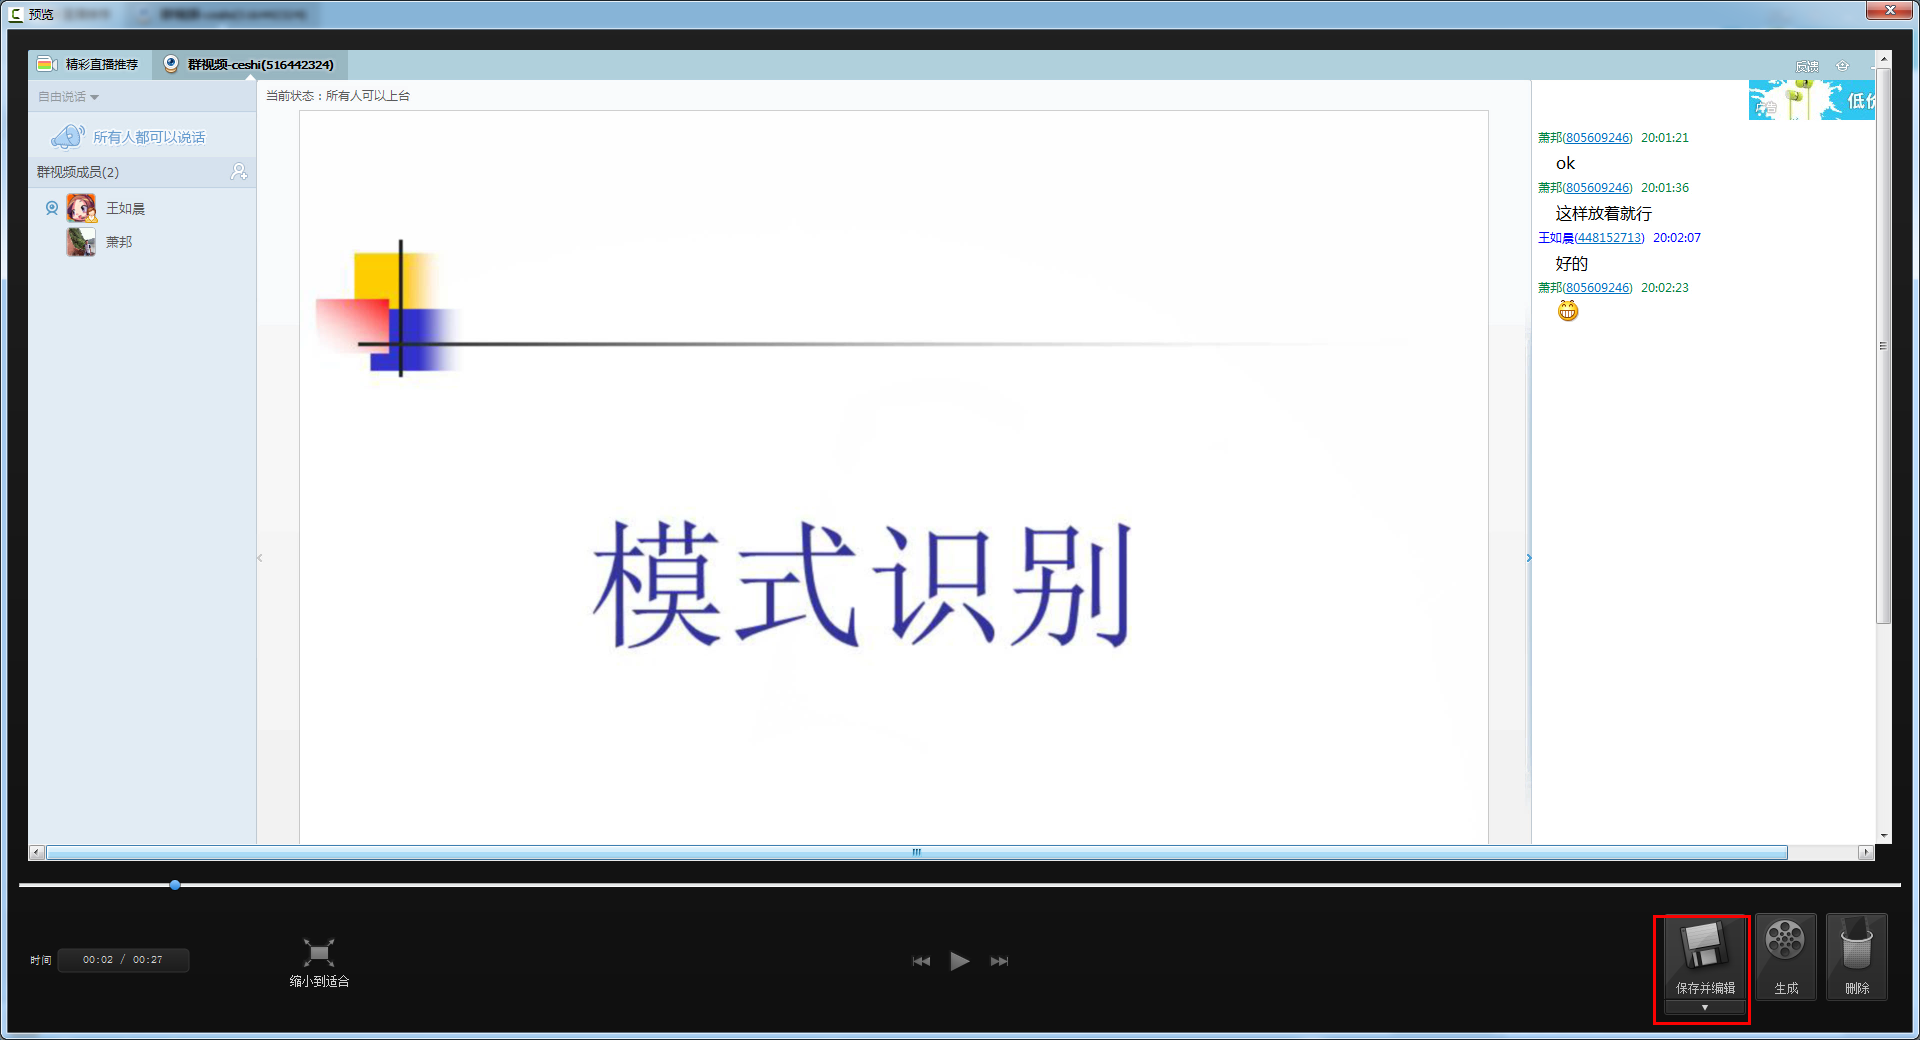
\includegraphics[width=0.9\textwidth]{fig4.png}
    \caption{保存录制文件}
    \label{fig:fig4}
    \end{figure} 
\section{导出mp4文件}\label{sec:daochu}
1. 选择{\color{blue}{编辑尺寸}},如图~\ref{fig:fig5}所示;选择{\color{blue}{1080p}},如图~\ref{fig:fig6}所示。\par
    \begin{figure}[!ht]
    \centering
    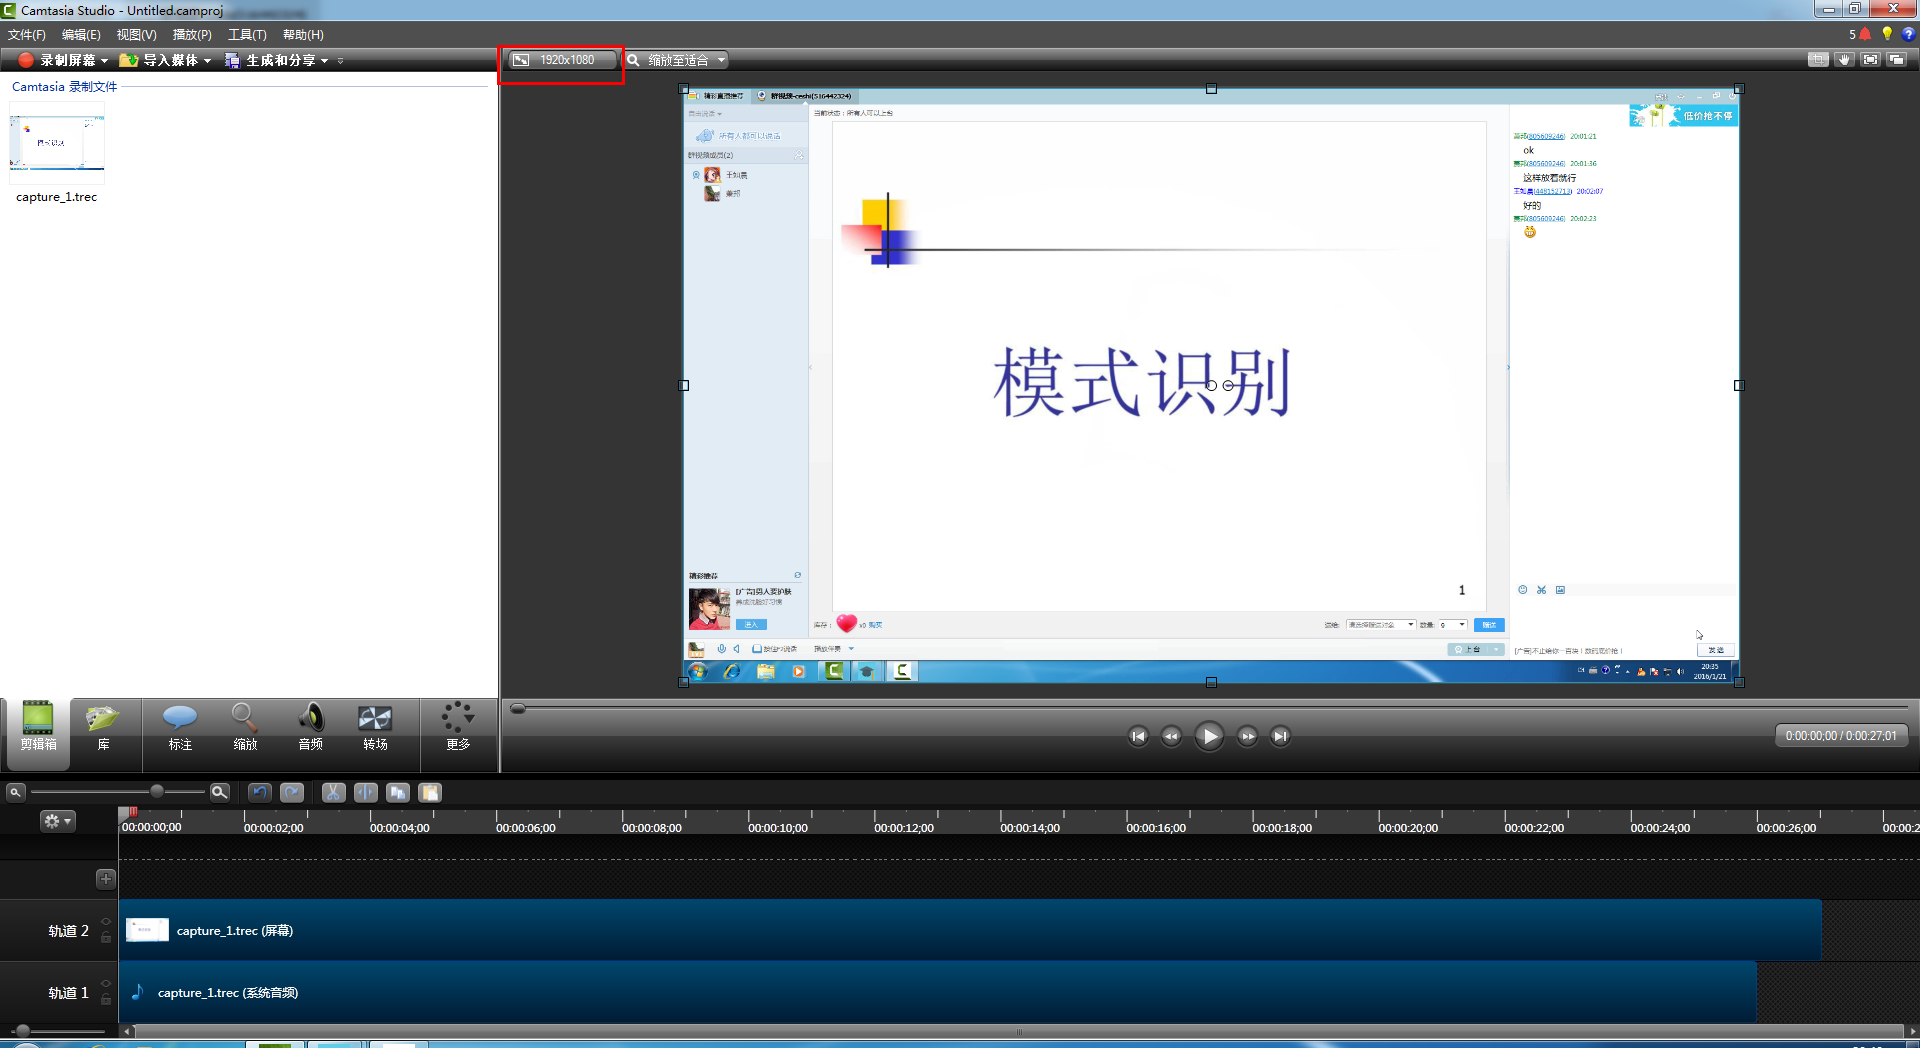
\includegraphics[width=0.9\textwidth]{fig5.png}
    \caption{点击编辑尺寸}
    \label{fig:fig5}
    \end{figure}
    \begin{figure}
    \centering
    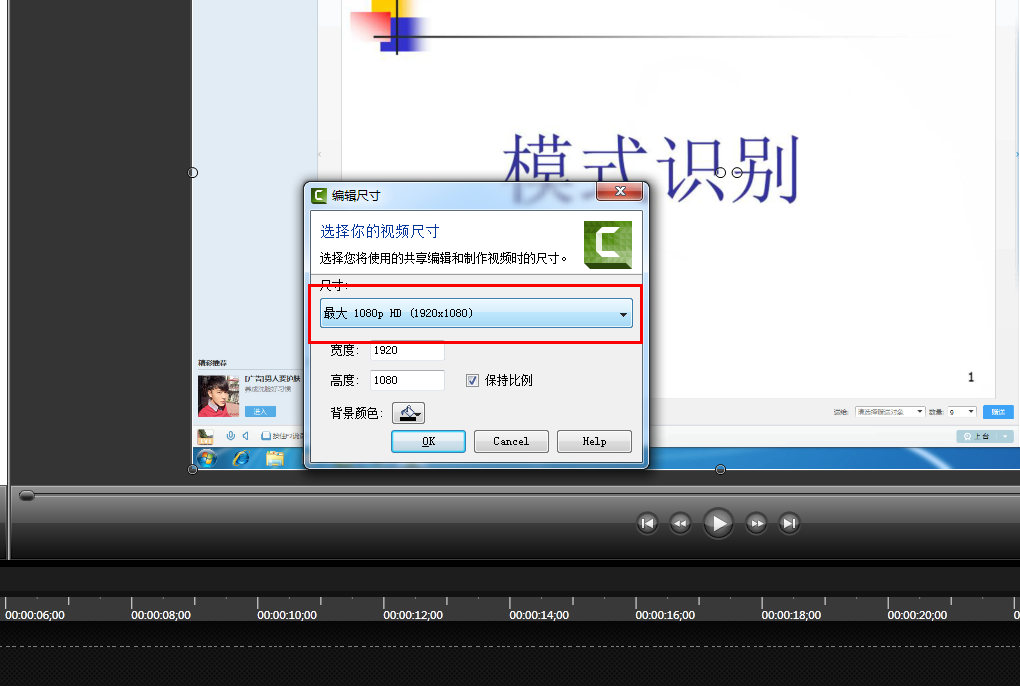
\includegraphics[width=0.9\textwidth]{fig6.png}
    \caption{选择编辑尺寸}
    \label{fig:fig6}
    \end{figure}
 %2. 点击{\color{blue}{“文件”-“保存项目”}},保存xxxx..camproj文件。\par
 2. 点击{\color{blue}{生成与分享}},如图~\ref{fig:fig7}所示。\par
     \begin{figure}
    \centering
    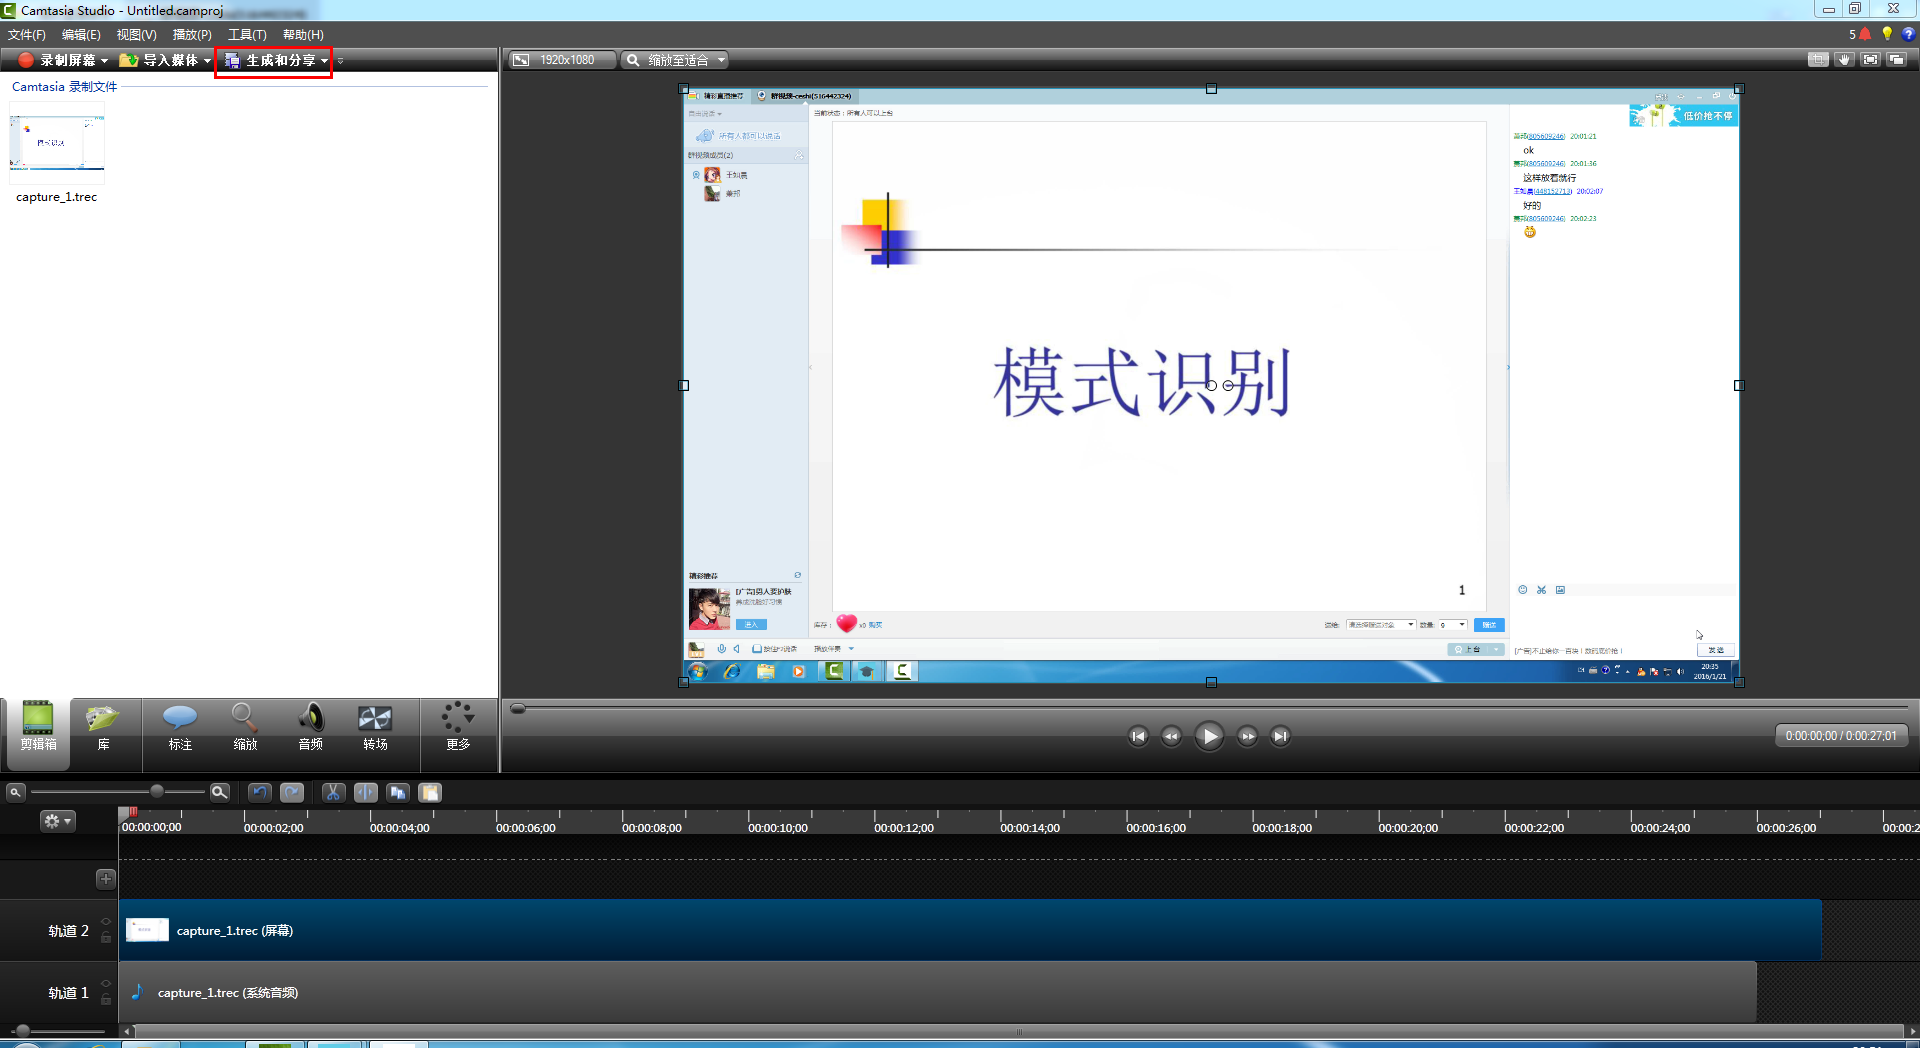
\includegraphics[width=0.9\textwidth]{fig7.png}
    \caption{生成mp4文件}
    \label{fig:fig7}
    \end{figure}
3. 选择如图~\ref{fig:fig8}的导出的mp4文件的参数。\par
     \begin{figure}
    \centering
    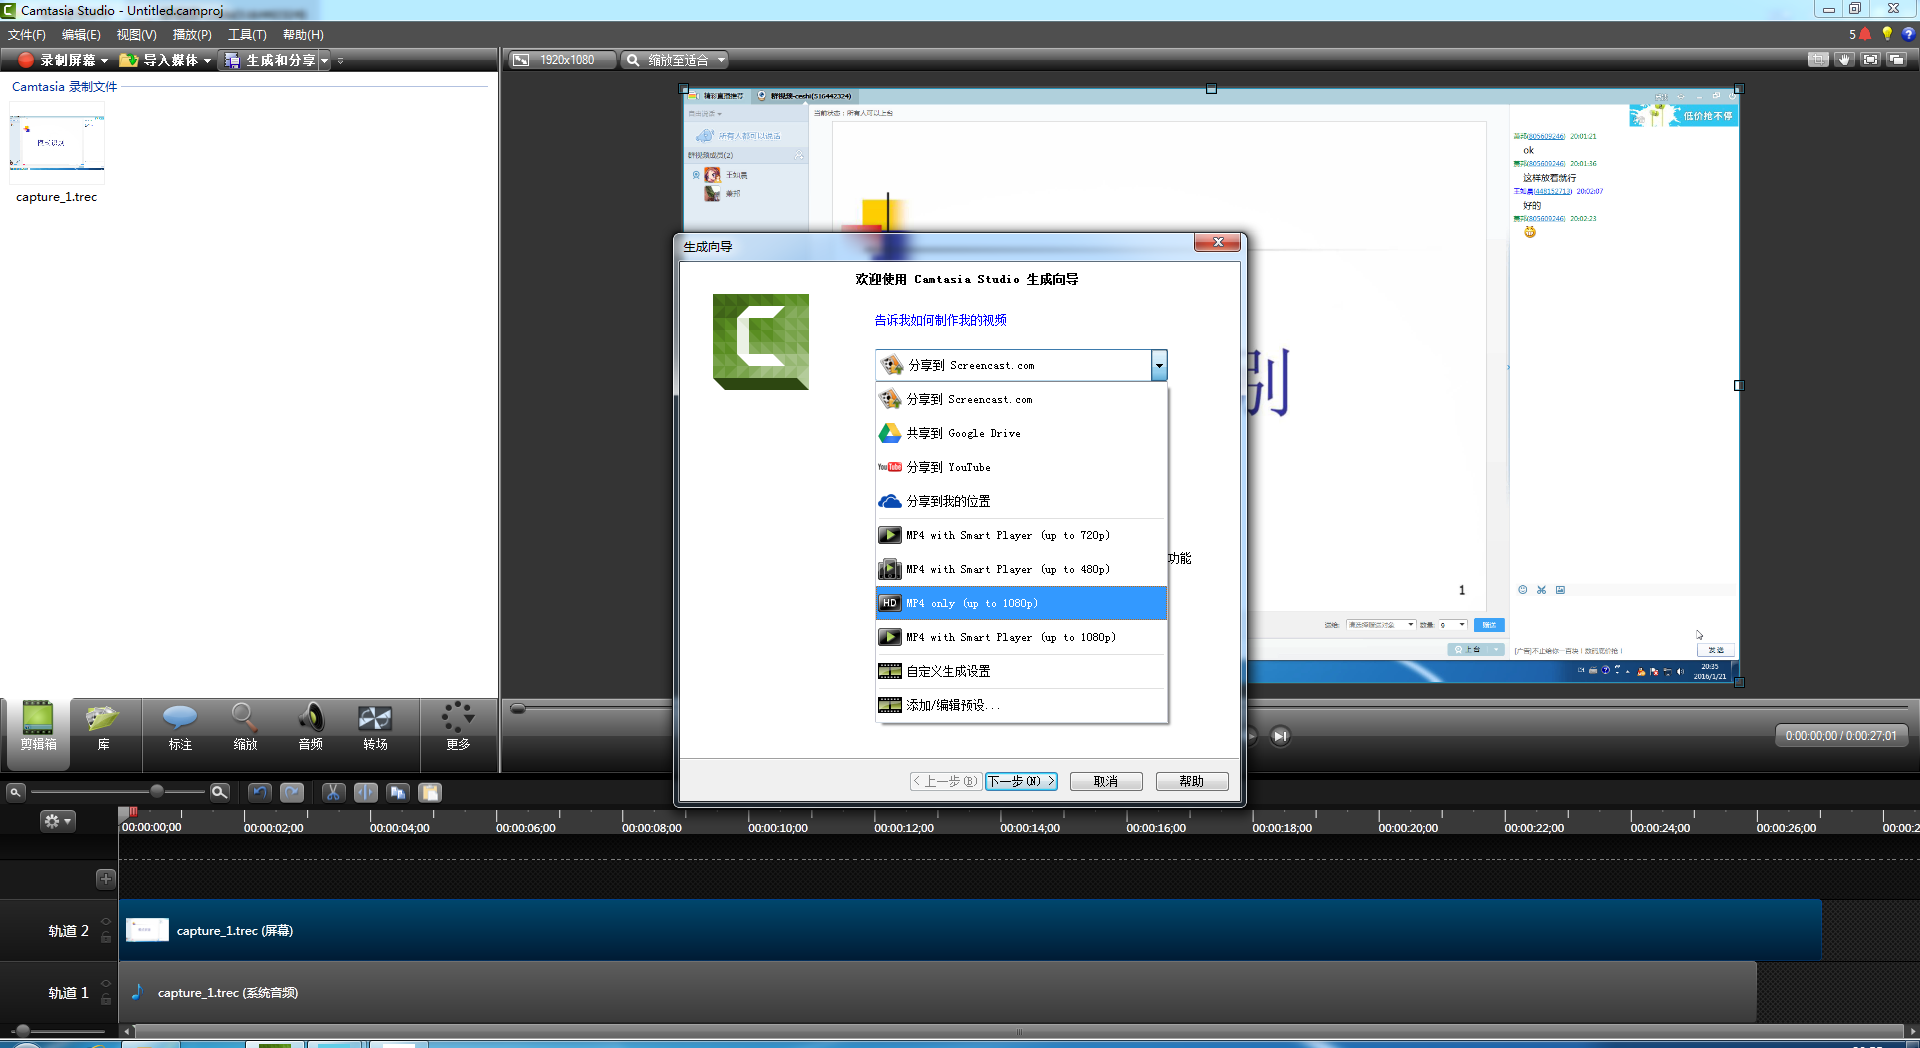
\includegraphics[width=0.9\textwidth]{fig8.png}
    \caption{生成mp4文件的参数}
    \label{fig:fig8}
    \end{figure}
4. 选择如图~\ref{fig:fig9}所示保存mp4文件的输出路径。\par
     \begin{figure}
    \centering
    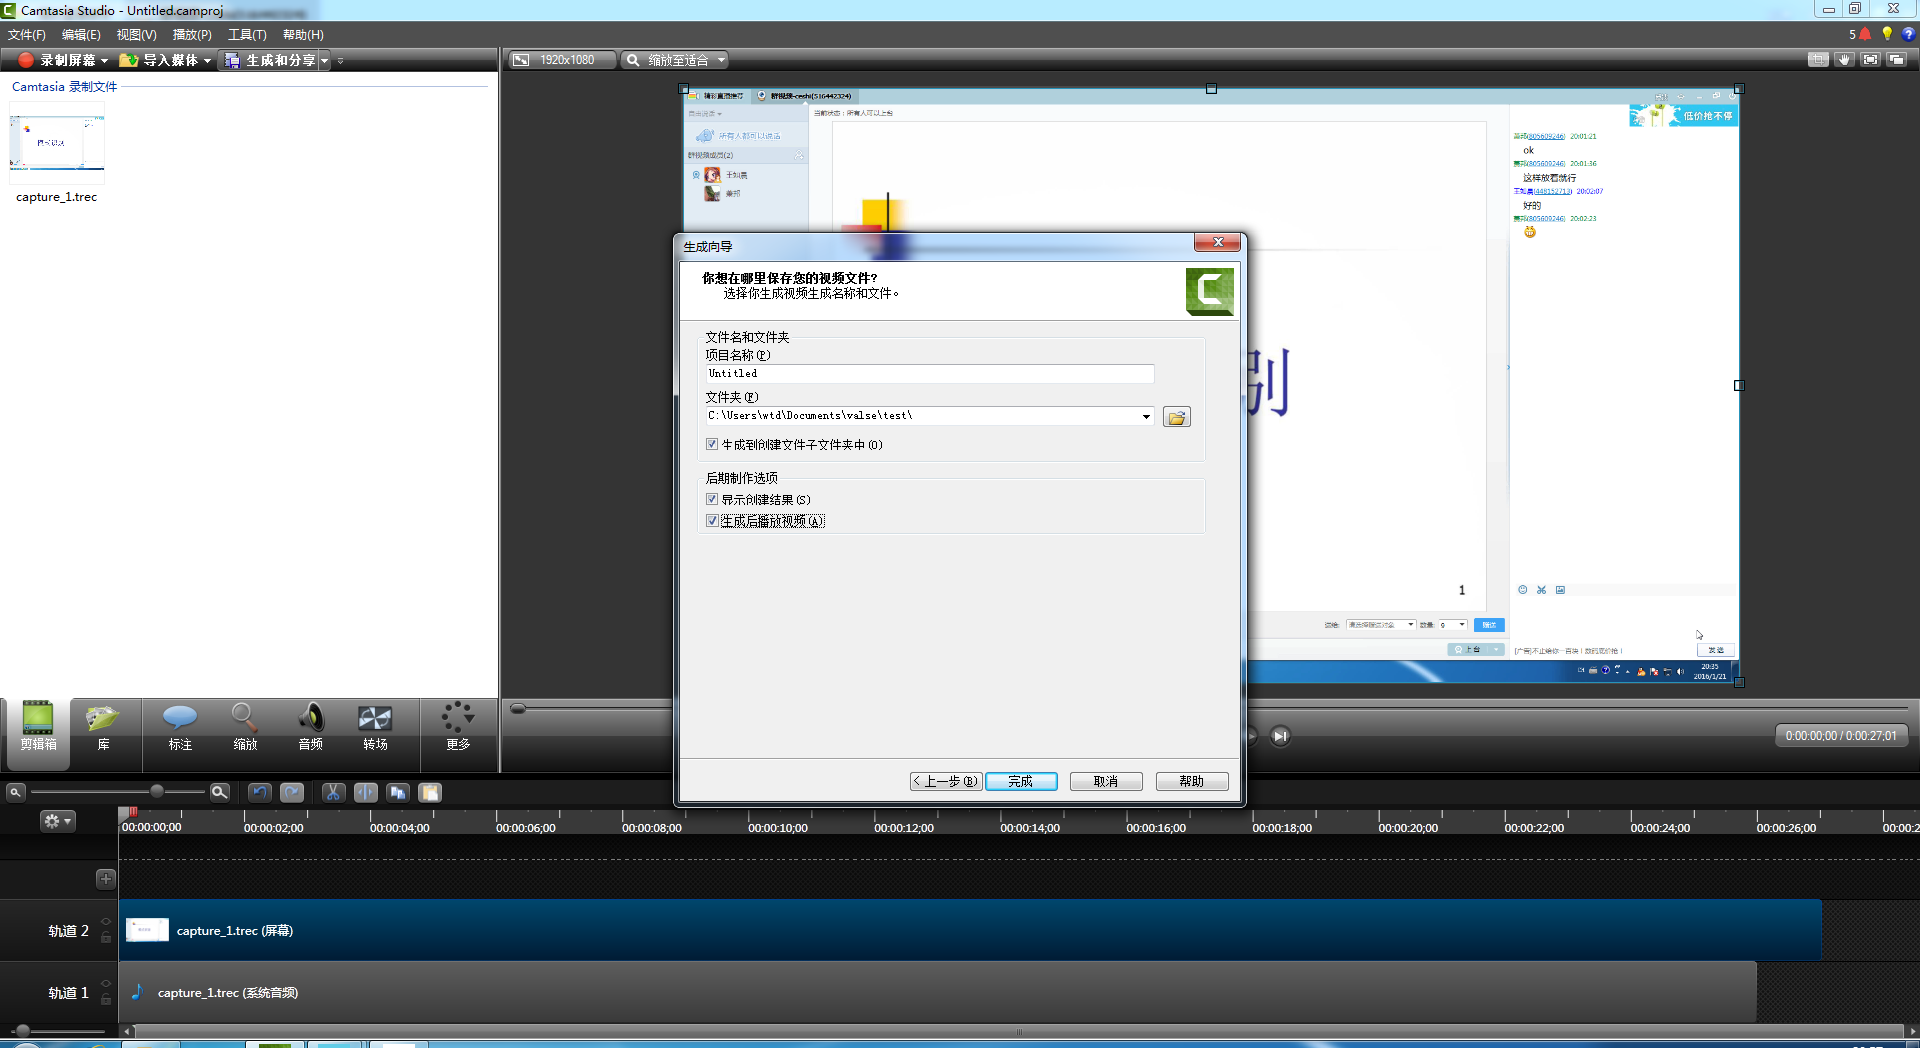
\includegraphics[width=0.9\textwidth]{fig9.png}
    \caption{设置mp4文件的生成路径}
    \label{fig:fig9}
    \end{figure}
5. xxxx.mp4文件正在生成如图~\ref{fig:fig10}所示。
     \begin{figure}
    \centering
    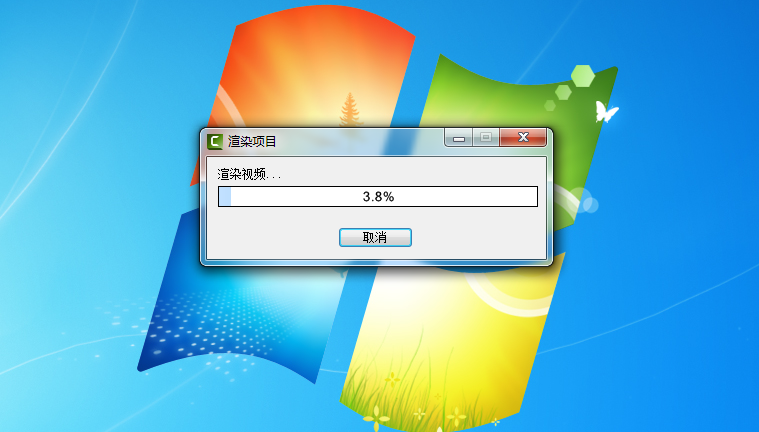
\includegraphics[width=0.9\textwidth]{fig10.png}
    \caption{mp4文件生成中}
    \label{fig:fig10}
    \end{figure}
\section{裁剪视频}
1. 点击Camtasia Studio软件右上角的{\color{blue}{裁剪按钮}},如图~\ref{fig:fig11}所示。\par
     \begin{figure}
    \centering
    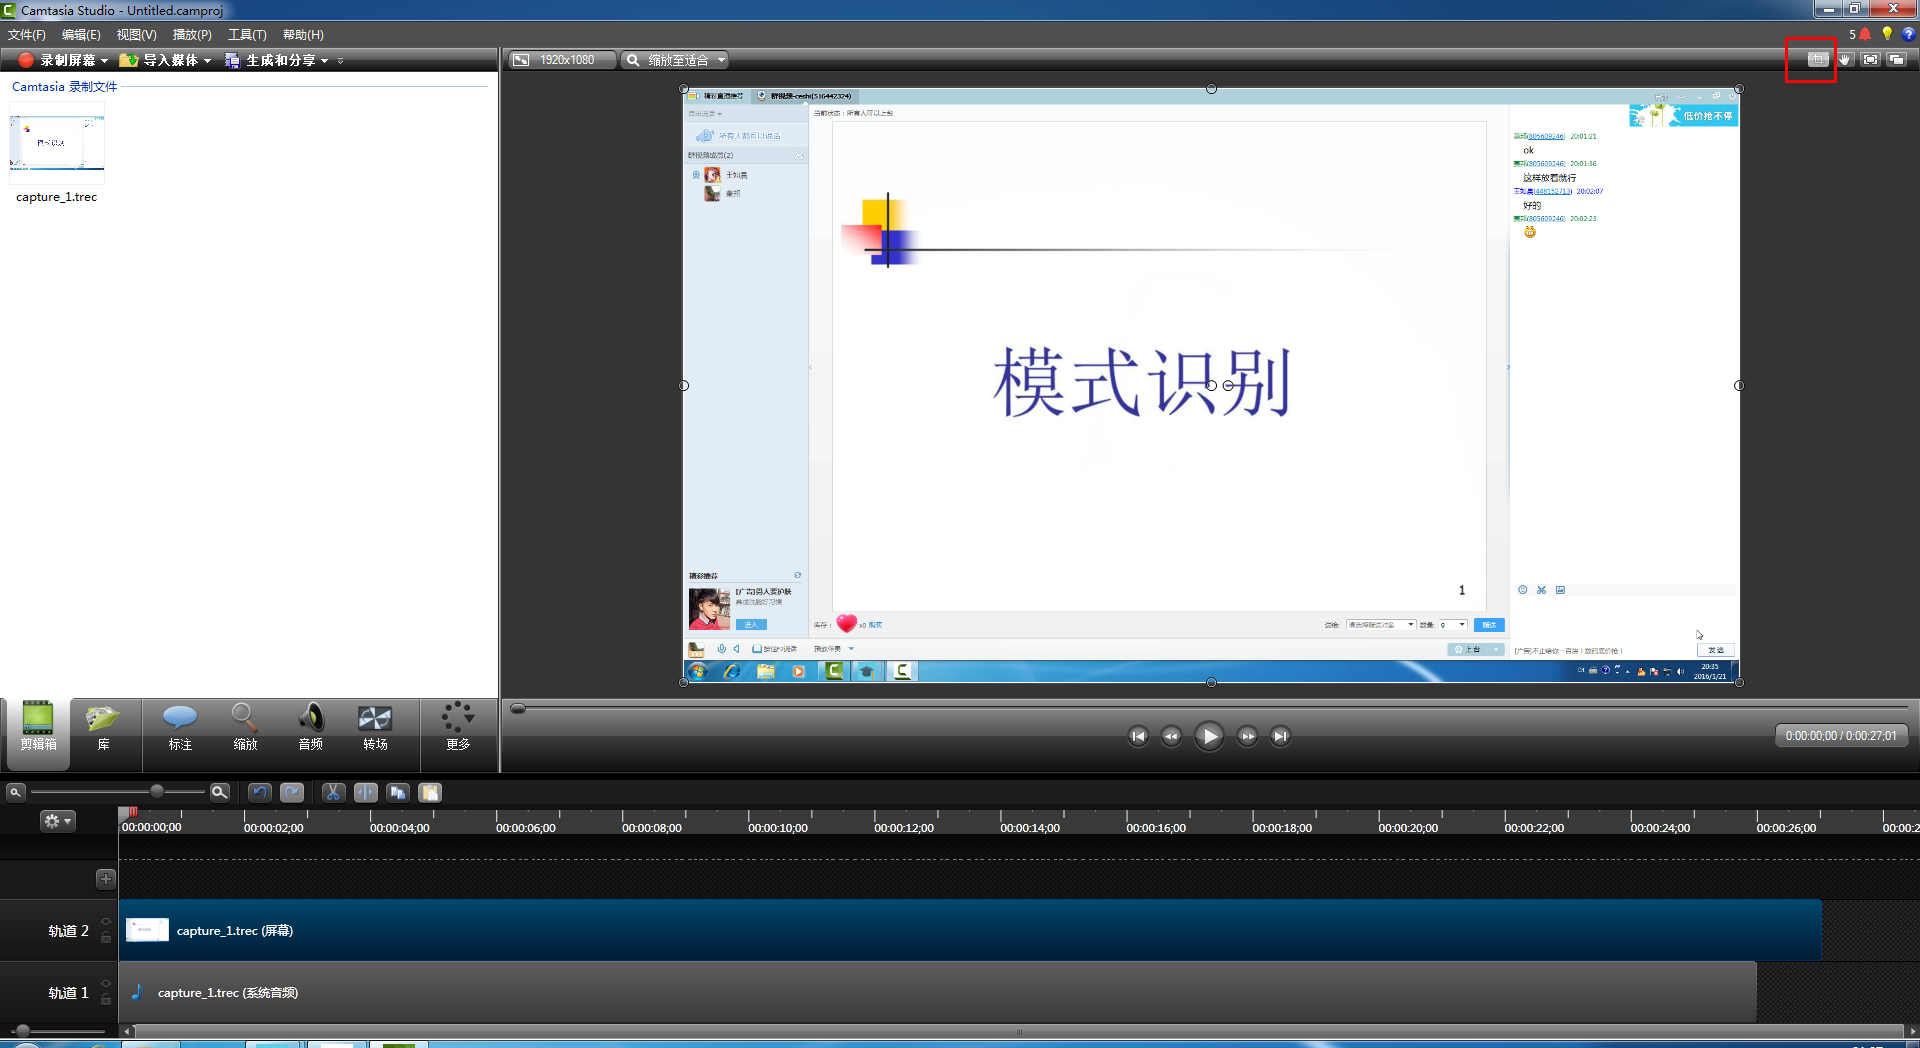
\includegraphics[width=0.9\textwidth]{fig11.png}
    \caption{点击裁剪按钮}
    \label{fig:fig11}
    \end{figure}
2. 拖拽视频框的小方块,只留{\color{blue}{ppt部分}},如图~\ref{fig:fig12}所示。\par
     \begin{figure}
    \centering
    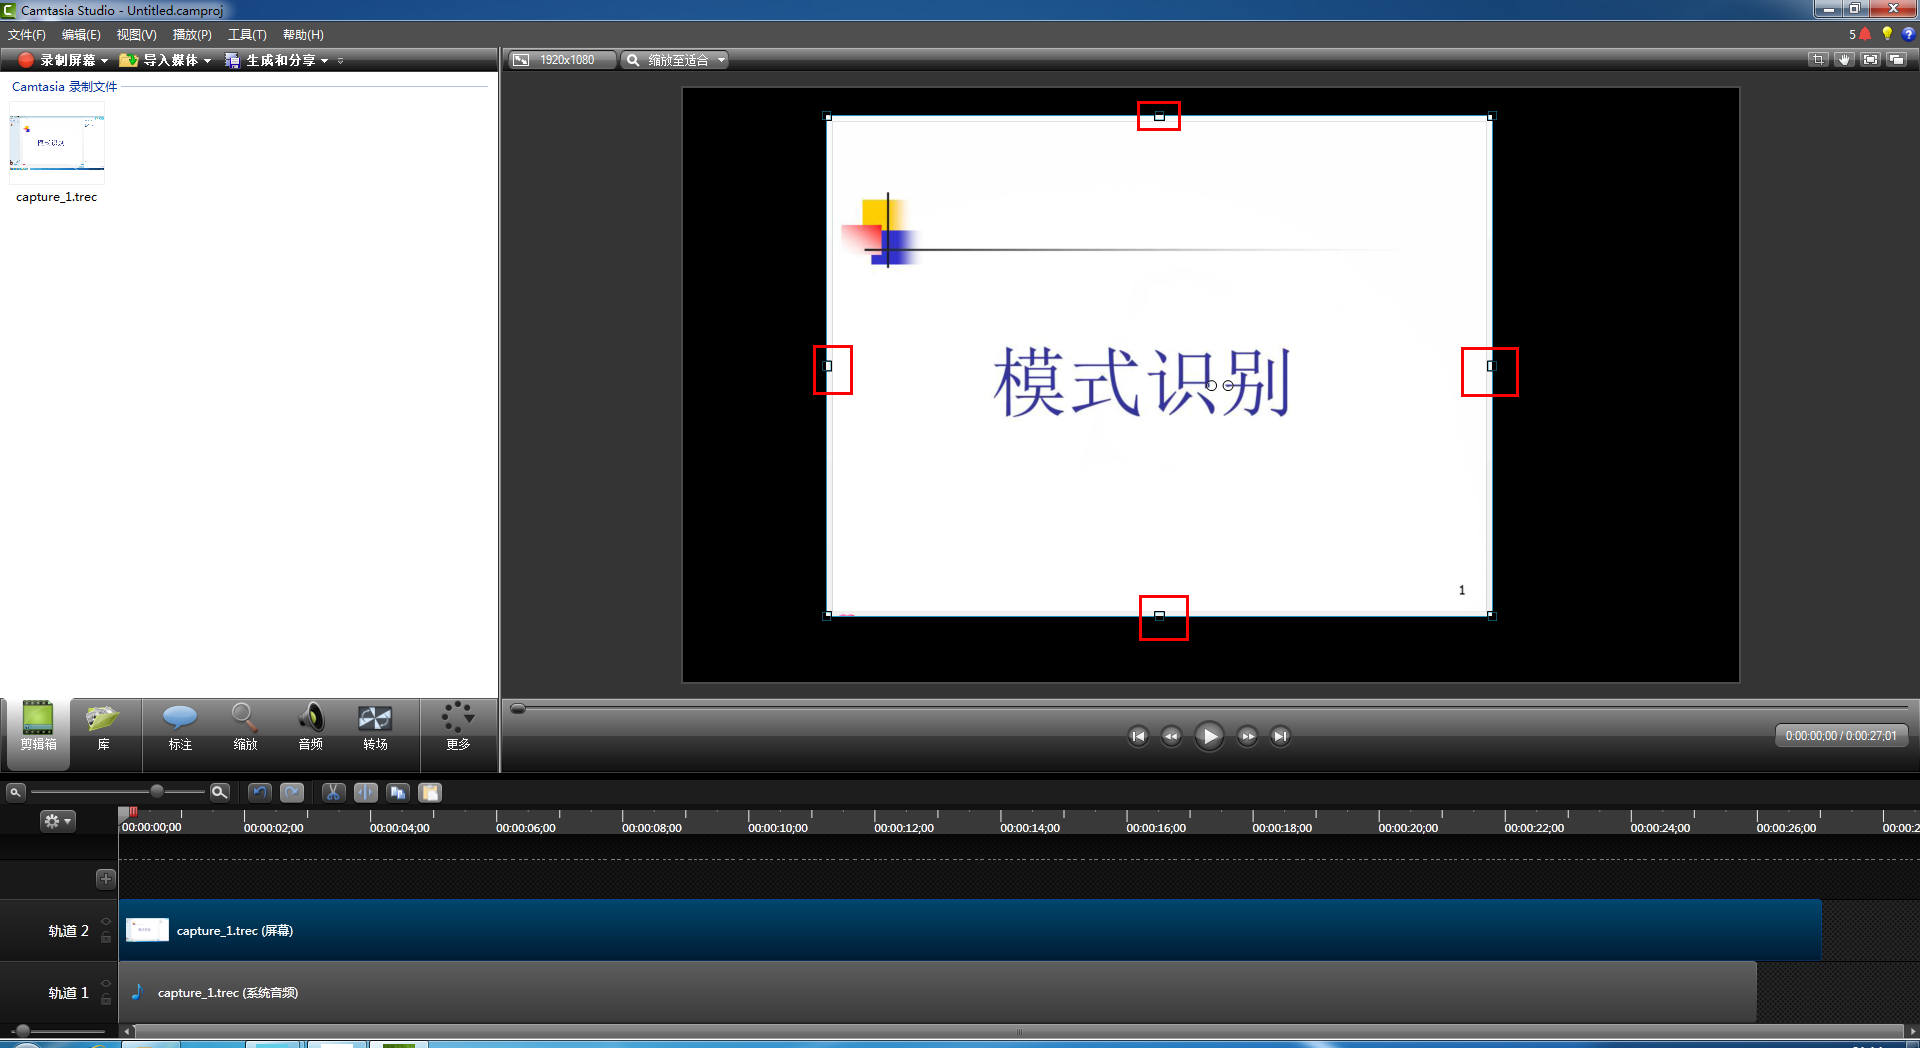
\includegraphics[width=0.9\textwidth]{fig12.png}
    \caption{调整视频尺寸大小}
    \label{fig:fig12}
    \end{figure}
3. 再点击右上角的裁剪按钮,拖拽视频框右下角的小圆圈(如图~\ref{fig:fig13}),使得视频等比例放大(上下不留黑边、左右可有黑边),并左右移动视频使其处于正中央,如图~\ref{fig:fig14}所示。\par
     \begin{figure}
    \centering
    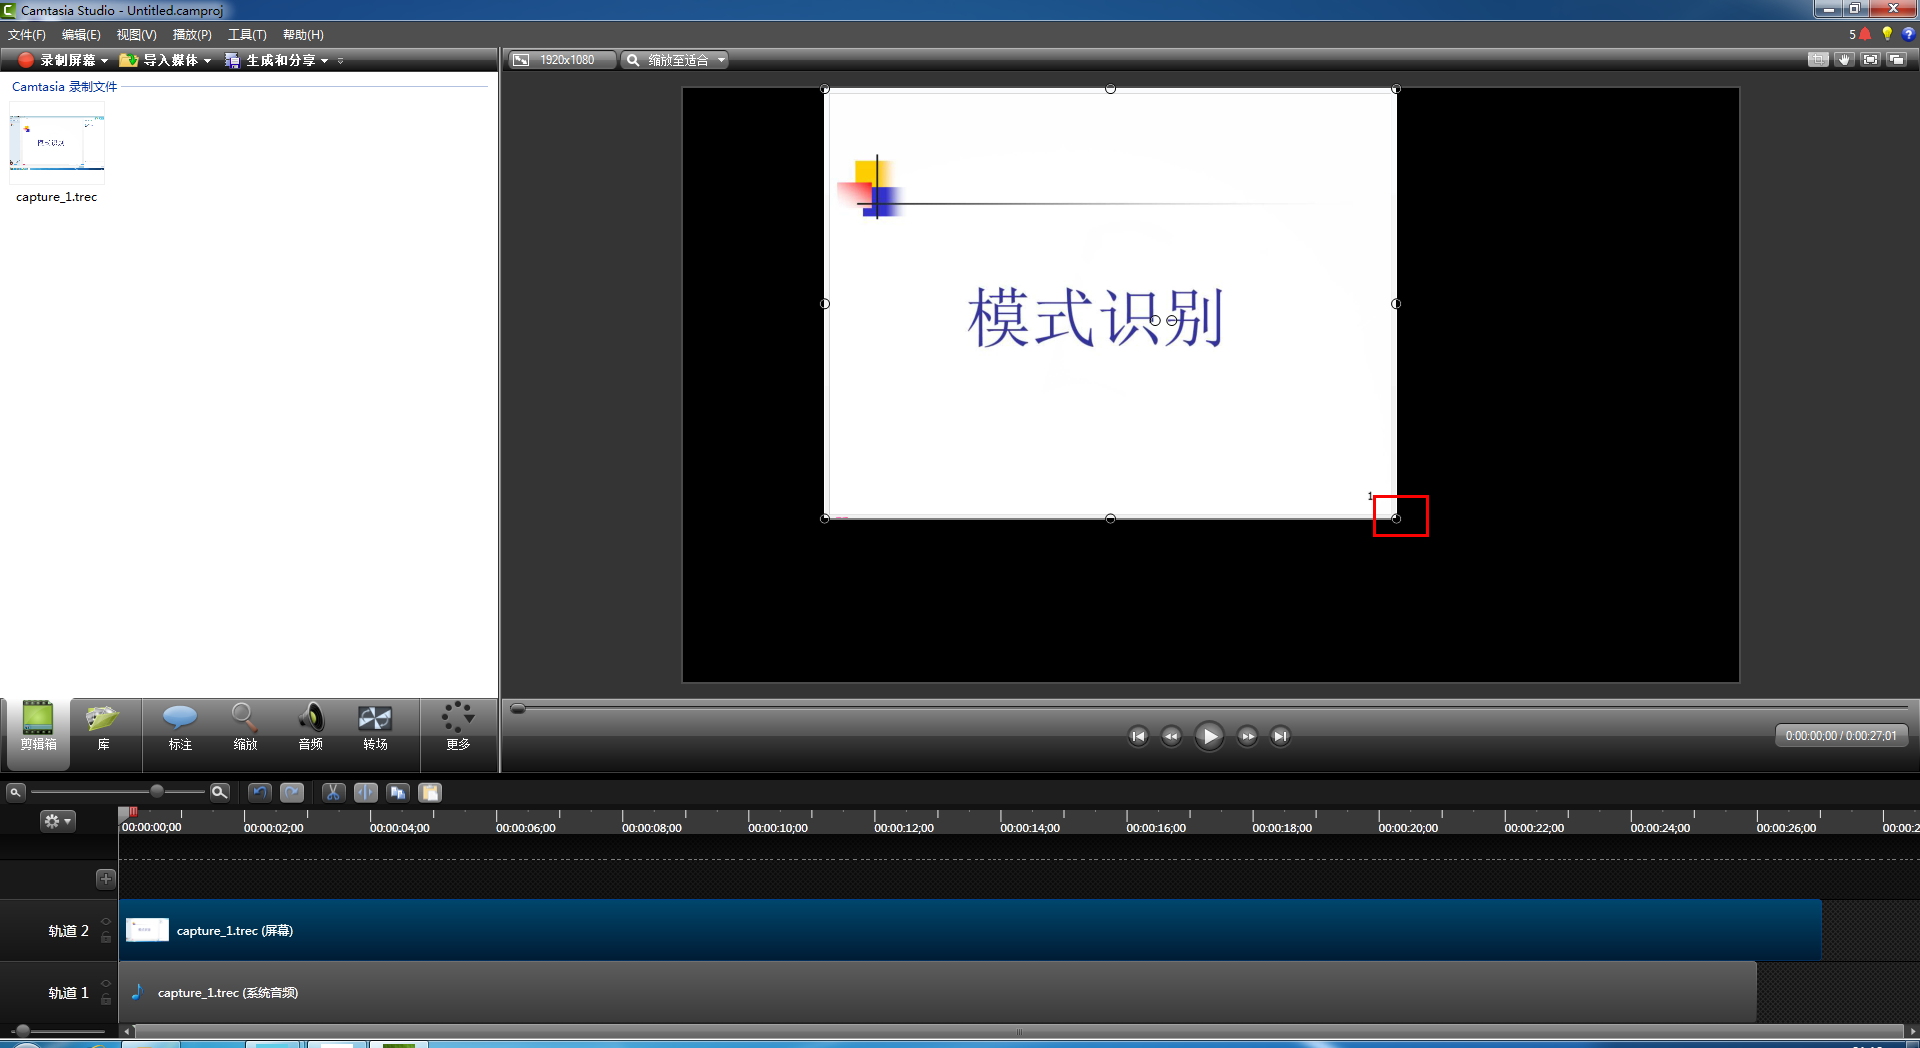
\includegraphics[width=0.9\textwidth]{fig13.png}
    \caption{调整视频尺寸大小}
    \label{fig:fig13}
    \end{figure}
         \begin{figure}
    \centering
    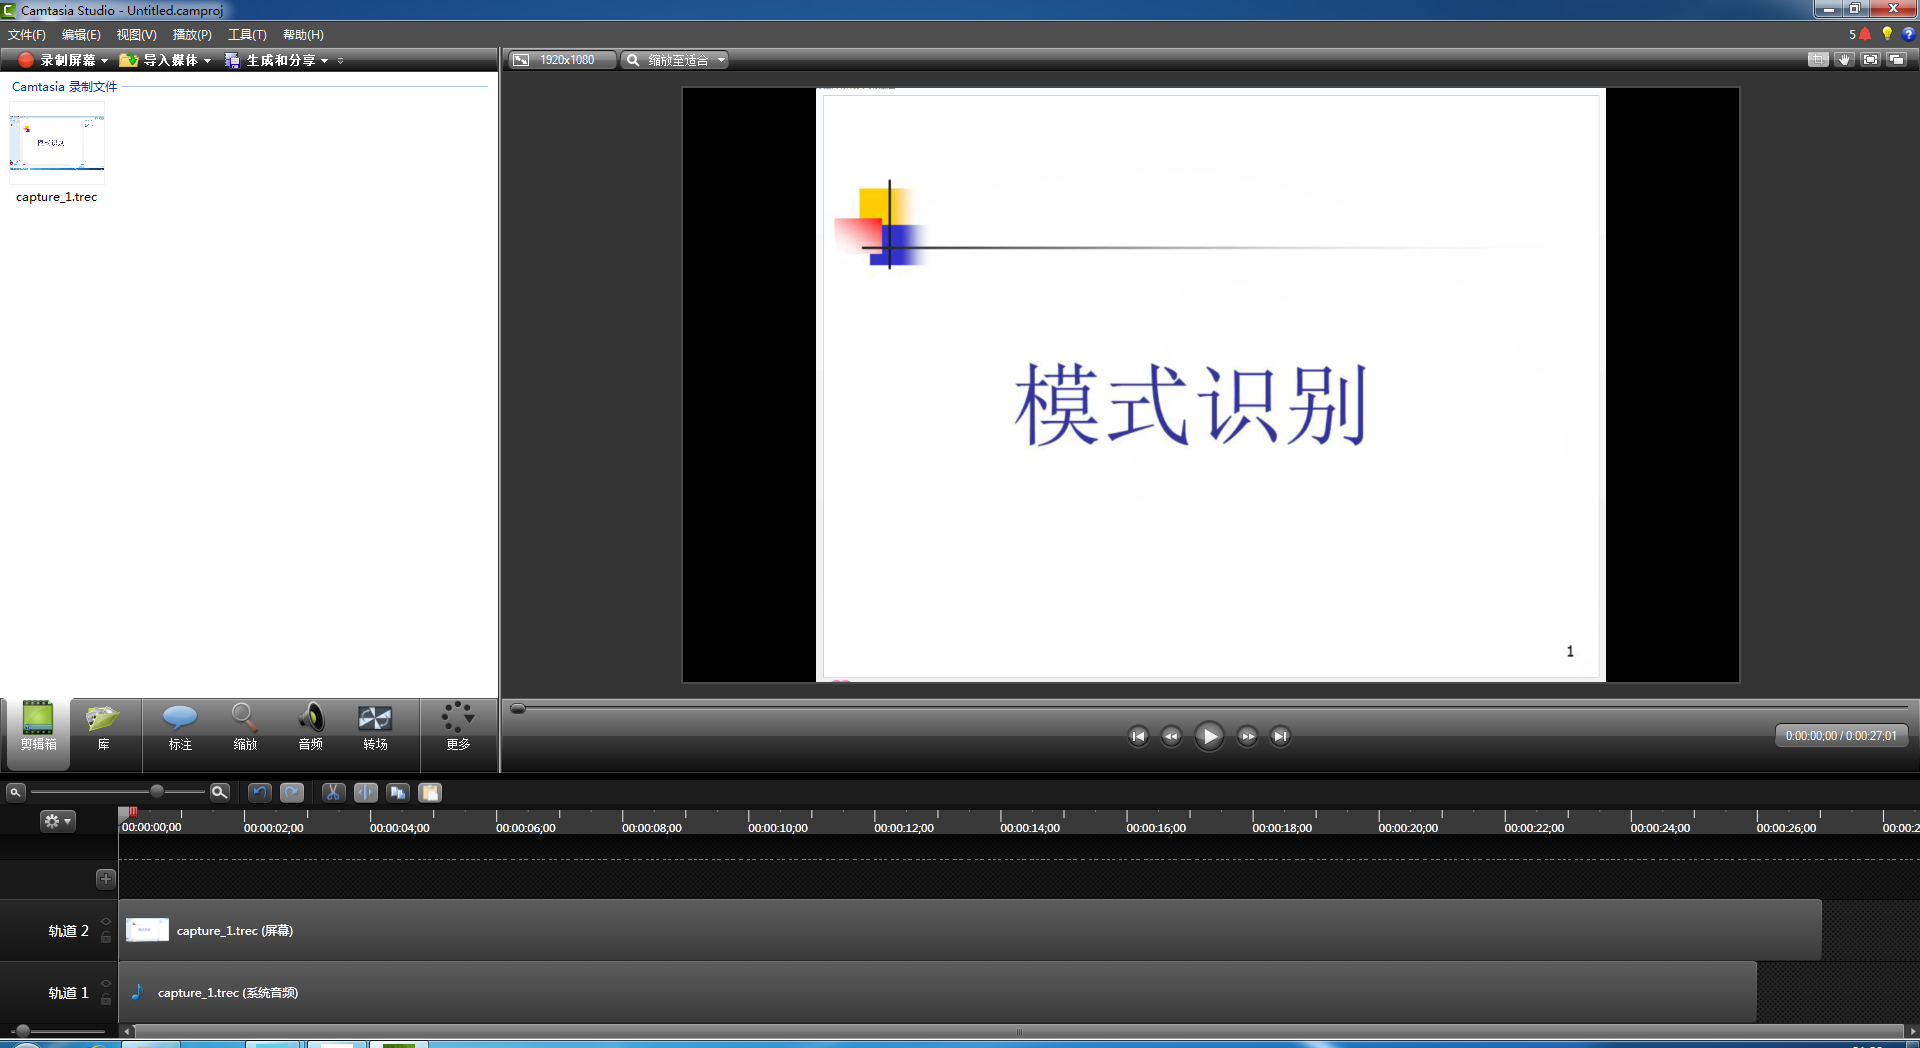
\includegraphics[width=0.9\textwidth]{fig14.png}
    \caption{调整视频尺寸大小}
    \label{fig:fig14}
    \end{figure}
4. 按照Section~\ref{sec:daochu}导出mp4文件。\\
{\color{blue}{注}}:原始视频和裁剪后的视频都需要生成及保存。



%%---------------------------------------------------------------------
\end{document}
